\documentclass[aspectratio=169]{beamer}

% Je kan het lettertype iets vergroten door hierboven optie ``14pt'' toe te
% voegen.

%==============================================================================
% Aanloop
%==============================================================================

%---------- Vormgeving --------------------------------------------------------

\usetheme{hogent}

% Kies hieronder een achtergrondkleur
%\usecolortheme{hgwhite} % witte achtergrond, zwarte tekst
\usecolortheme{hgblack} % zwarte achtergrond, witte tekst

%---------- Packages ----------------------------------------------------------

\usepackage[english]{babel}      % Nederlandse taal: splitsingen, enz.

\usepackage{booktabs}          % Mooie tabellen
\usepackage{multirow,multicol} % Tabelcellen samenvoegen
\usepackage{eurosym}           % Euro symbool

%\usepackage{animate} % GIFS
\usepackage{media9}
\usepackage{fontspec}
\usepackage{multimedia} % Use multimedia instead of media9



%---------- Commando-definities -----------------------------------------------

%---------- Info over de presentatie ------------------------------------------

\title[AI Judge]{AI judge assistant for recognition of jump rope skills in videos.}
\author{Mike De Decker}
\author[MDD]{Mike {De Decker} (\href{mailto:mikeddecker@hotmail.com}
    {mikeddecker@hotmail.com})}
\date{\today}

%==============================================================================
% Inhoud presentatie
%==============================================================================

\begin{document}

%---------- Titelpagina, inhoudstafel -----------------------------------------

{
\setbeamertemplate{background}[imgletter]
    {dd3-boxes-dark.jpg}{H}

\begin{frame}
    \maketitle
\end{frame}
}

%---------- Corpus ------------------------------------------------------------

\begin{frame}
  \frametitle{Diciplines}

  \hspace{0.1cm}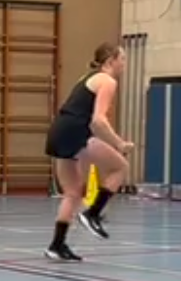
\includegraphics[height=2cm]{speed}
  \hspace{0.1cm}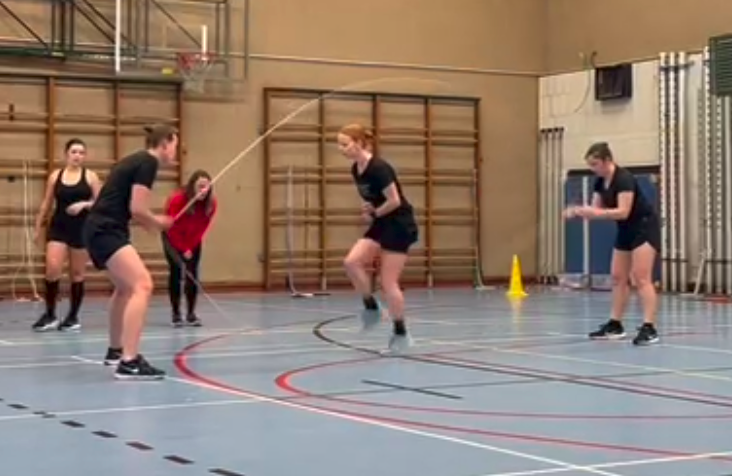
\includegraphics[height=2cm]{ddspeed}
  \hspace{0.1cm}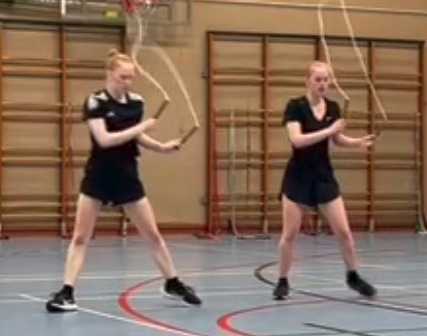
\includegraphics[height=2cm]{sr}
  \hspace{0.1cm}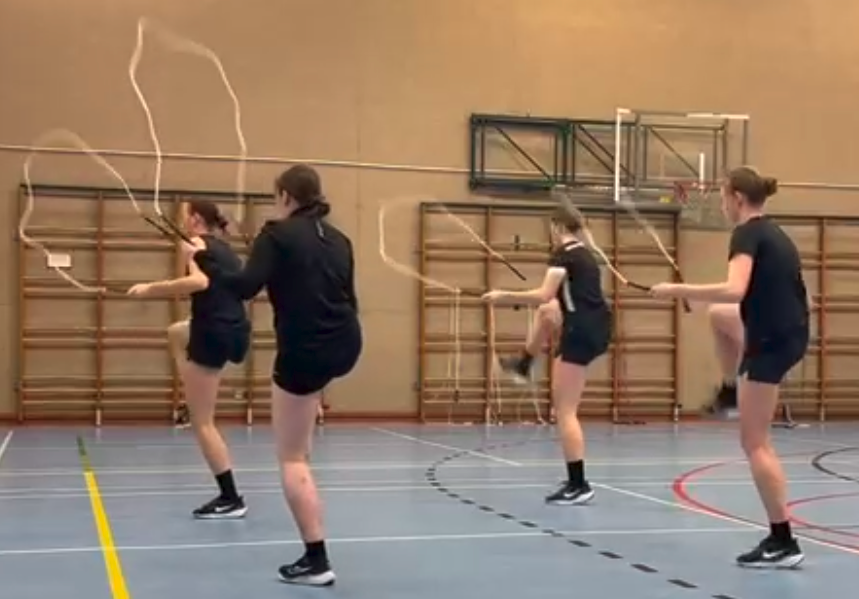
\includegraphics[height=2cm]{sr-team} \\
  \vspace{0.1cm}
  \hspace{0.1cm}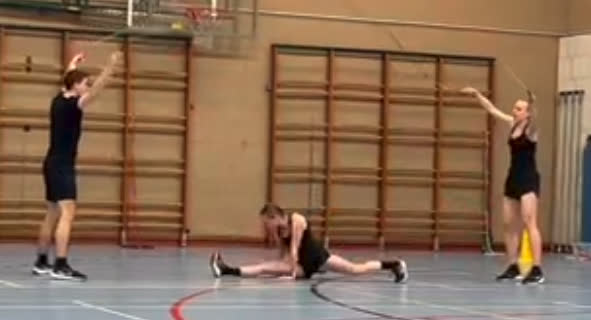
\includegraphics[height=2cm]{dd3}
  \hspace{0.1cm}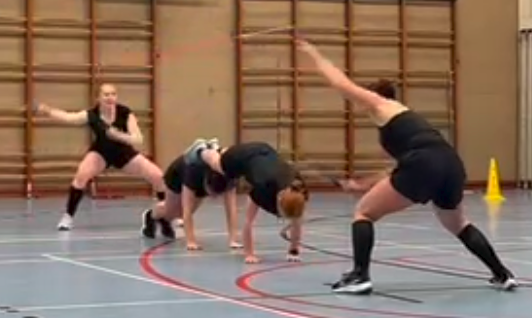
\includegraphics[height=2cm]{dd4}
  \hspace{0.1cm}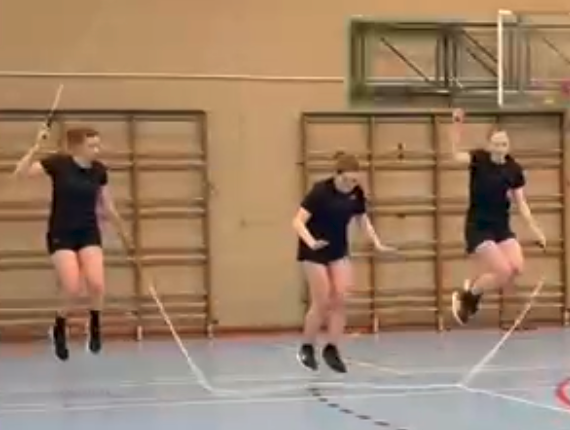
\includegraphics[height=2cm]{cw}

\end{frame}

\begin{frame}{Video example}
  % \frametitle{Comparing routines - GIFS}

  % \movie[width=0.8\linewidth,height=0.6\linewidth,poster,autostart]{Click to play}{sr2-zoe-elena.mov}
  % \includemedia[
  %     activate=pageopen,
  %     width=0.8\linewidth,
  %     height=0.6\linewidth,
  %     addresource=graphics/2024-dd3-sipiro-maud.mp4,
  %     flashvars={source=graphics/2024-dd3-sipiro-maud.mp4}
  % ]{}{VPlayer.swf}

  \href{run:1315_annotated.mp4}{Click to play the video}

  
  % 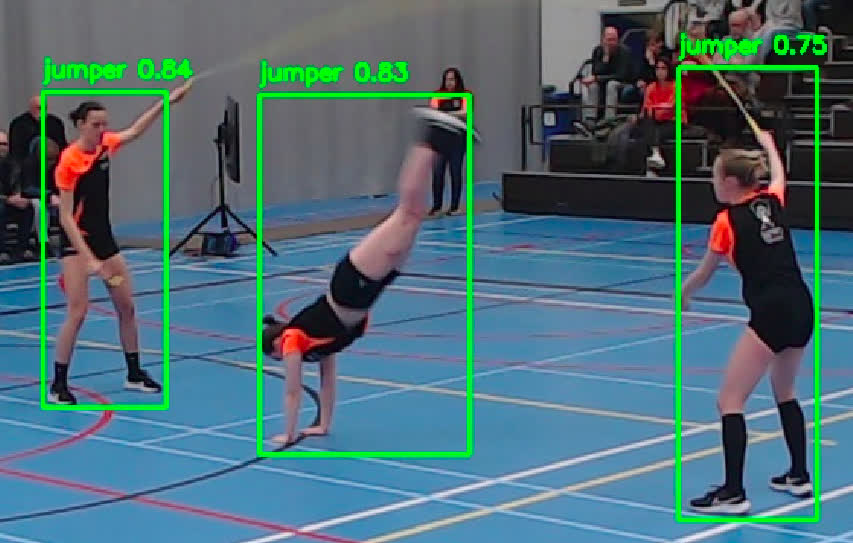
\includegraphics[height=4cm]{dd3-boxes.jpg}
  % 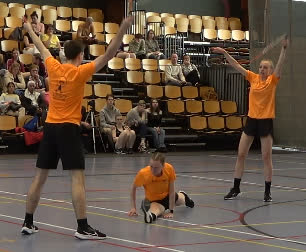
\includegraphics[height=4cm]{dd3-split.jpg}

\end{frame}

\begin{frame}
  \frametitle{Judges}
  \vspace{-1cm}
  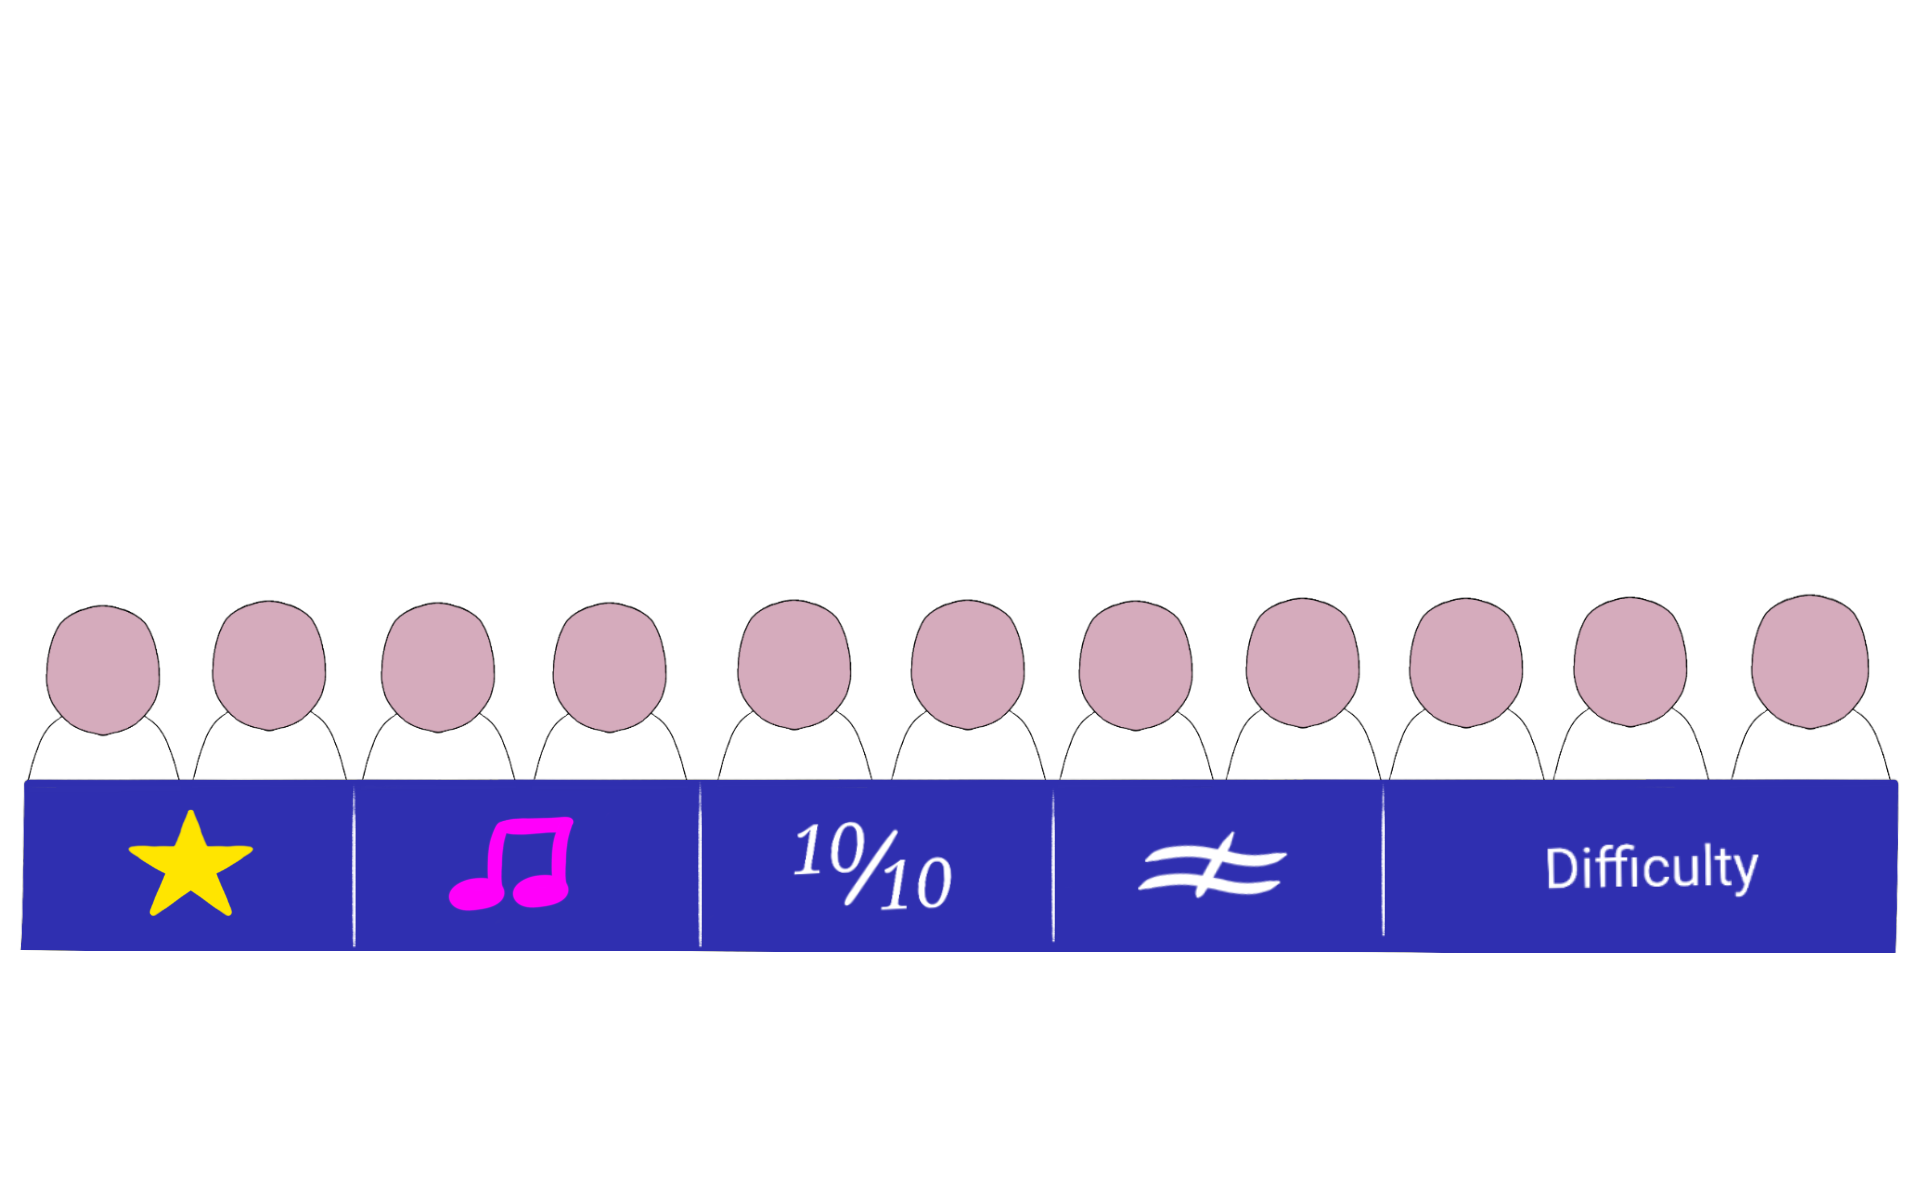
\includegraphics[width=0.9\linewidth]{judges}
  
  % TODO : add cine diffusion link if kept
\end{frame}

\begin{frame}
  \frametitle{Scoring difficulty.}
  \vspace{-0.3cm}
  Using levels [1 -> 8]
  \vspace{0.2cm}

  \begin{columns}[c]
  
    \column{.55\textwidth}
    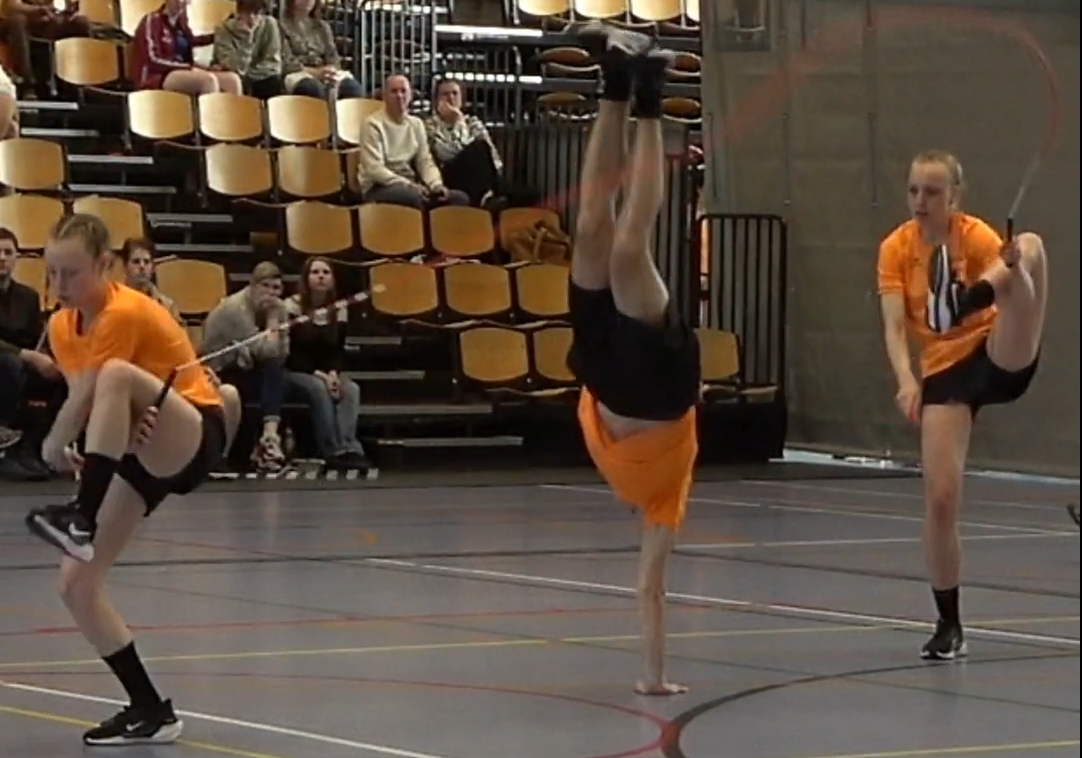
\includegraphics[width=0.9\linewidth]{dd3-1h-hfrog-toad-bw-crouger}

    \column{.45\textwidth}
    Base skill level \\
    + \\
    Turner restrictions \\
    + \\
    Nr of rotations \\
    + \\
    Modifiers (one hand, body rotations...)

  \end{columns}
\end{frame}

\begin{frame}
  \frametitle{AI Judge assistant}

  \begin{columns}[c]
  
    \column{.65\textwidth}
    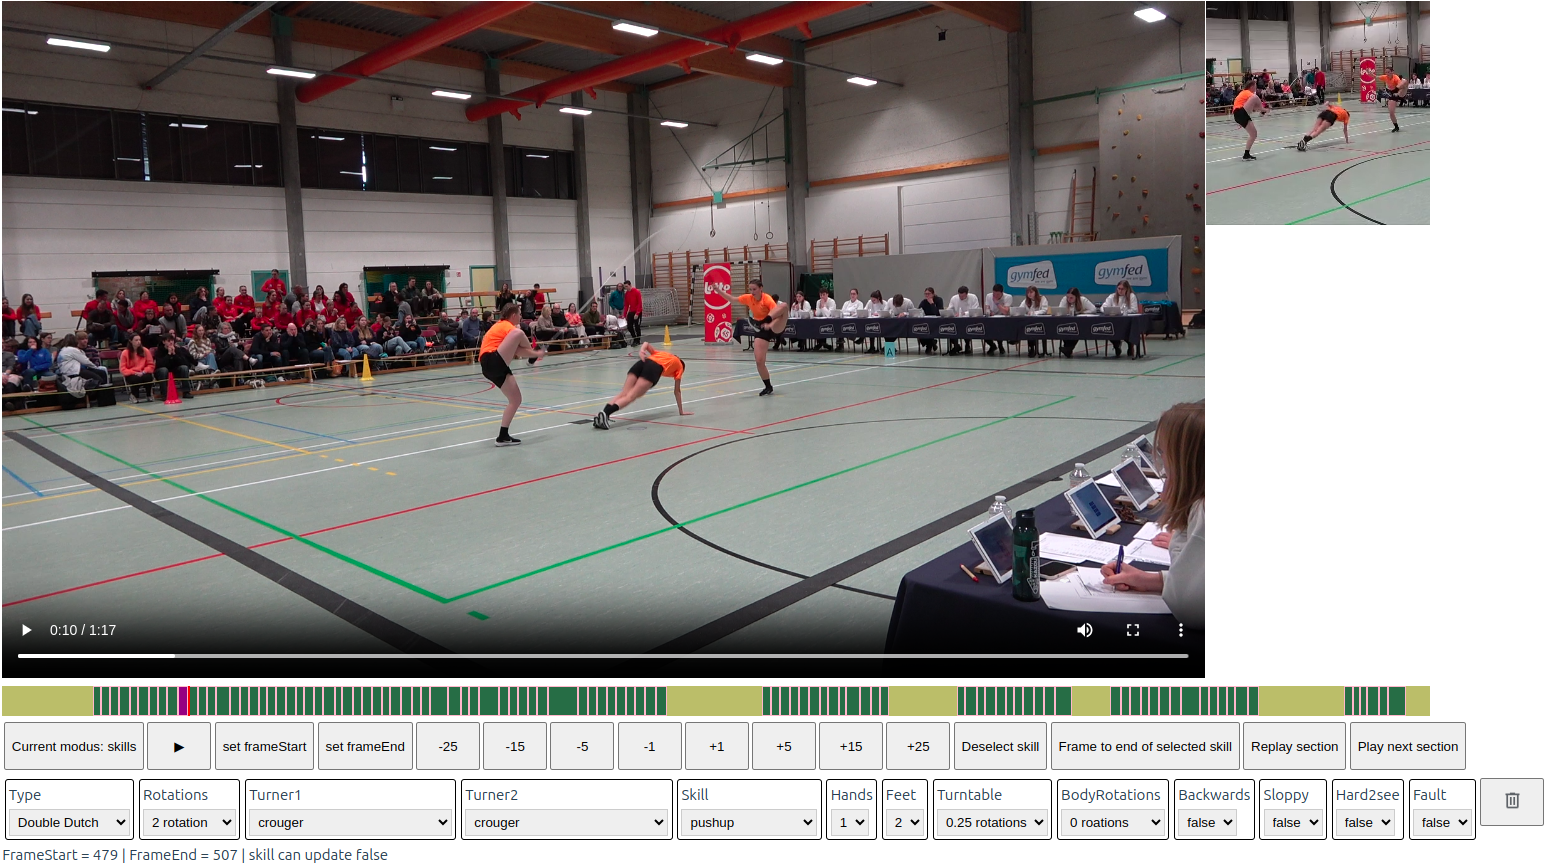
\includegraphics[width=0.9\linewidth]{label-video}

    \column{.35\textwidth}
    \begin{enumerate}
      \item localize
      \item segment
      \item recognition
    \end{enumerate}

  \end{columns}
\end{frame}

\begin{frame}
  \frametitle{AI Judge assistant}

  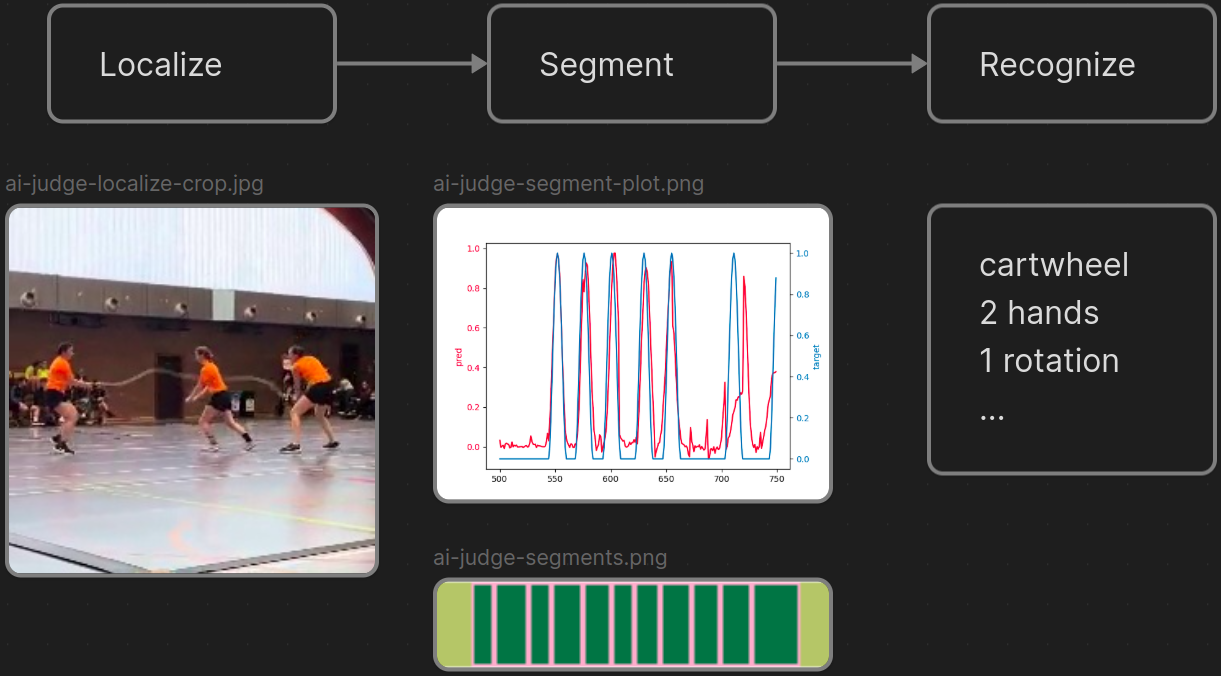
\includegraphics[width=0.8\linewidth]{flow}

\end{frame}


\end{document}
